\newpage
\section{降维与度量学习}
\subsection{k近邻学习(kNN)}
k-Nearest Neighbor. 给定测试样本,基于某种距离度量找出训练集中与其最靠近的k
个训练样本,然后基于这k 个"邻居"的信息来进行预测

没有显式的训练过程. 

最近邻分类器虽简单,但它的泛化错误率不超过贝叶斯最优分类器的错误率的两倍.  

\subsection{低维嵌入}
维数灾难(curse of dimensionality) :在高维情形下出现的数据样本稀疏、距离计算困难等问题. 

维数约简(降维):通过某种数学变换将原始高维属性空间转变为一个低维“子空间”(subspace) ,在这个子空间中样本密度大幅提高, 距离计算也变得更为容易。

多维缩放:要求原始空间中样本之间的距离在低维空间中得以保持


对于降维后样本 $\bm Z$, 可通过降维前后保持不变的距离矩阵$\bm D$ 求取内积矩阵$\bm B=\bm {Z}^\top\bm {Z}$, 然后对 $\bm B$ 作特征值分解求 $\bm Z$. 

一般来说,欲获得低维子空间,最简单的是对原始高维空间进行线性变换
\begin{align*}
    \bm Z=\bm{W}^\top \bm X
\end{align*}
基于线性变换来进行降维的方法称为线性降维方法. 

\subsection{主成分分析(PCA)}
Principal Component Analysi. 对于正交属性空间中的样本点,用一个超平面(直线的高维推广)对所有样本进行恰当的表达. 
\begin{itemize}
    \item 最近重构性:样本点到这个超平面的距离都足够近
    \item 最大可分性:样本点在这个超平面上的投影能尽可能分开
\end{itemize}


\begin{figure}[!htb]
    \centering
    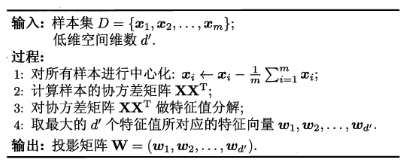
\includegraphics[width=0.42\textwidth]{pic/ML10/PCA 算法}
    \caption{PCA 算法}
\end{figure}


PCA 仅 需 保 留 $\bm W$ 与样本的均值向量即可通过简单的向量减法和矩阵-向
量乘法将新样本投影至低维空间中

\subsection{核化线性降维}
非线性阵维的一种常用方法,是基于核技巧对线性降维方法进行``核化''
\begin{align*}
    \bm{z}_i=\phi(\bx_i)
\end{align*}
$\phi$ 不能显示表示, 于是引入核函数
\begin{align*}
    \kappa(\bx_i,\bx_j)=\phi(\bx_i)^\top\phi(\bx_j)
\end{align*}

反正最后计算开销较大

\subsection{流形学习}
“流形”是在局部与欧氏空间同胚的空间,换言之,它在局部具有欧氏空间的性质,能用欧氏距离来进行距离计算。

若低维流形嵌入到高维空间中, 则数据样本在高维空间的分布虽
然看上去非常复杂,但在局部上仍具有欧氏空间的性质,因此,
可以容易地在局部建立阵维映射关系,然后再设法将局部映射关
系推广到全局。

两种著名的流形学习方法:
\begin{itemize}
    \item 等度量映射 (Isometric Mapping,简称Isomap)
    \item 局部线性嵌入 (Locally Linear Embedding,简称LLE)
\end{itemize}

\subsubsection{等度量映射(Isomap)}
计算测地线距离:
可利用流形在局部上与欧氏空间同胚这个性质,对每个点基于欧
氏距离找出其近邻点,然后就能建立一个近邻连接图,图中近邻
点之间存在连接,而非近邻点之间不存在连接, 于是,计算两点
之间测地线距离的问题就转变为计算近邻连接图上两点之间的最
短路径问题
\subsubsection{局部线性嵌入(LLE)}
试图保持邻域内样本之间的线性关系

\subsection{度量学习}
在机器学习中,对高维数据进行降维的主要目的是希望找一个合
适的低维空间,在此空间中进行学习能比原始空间性能更好。事
实上,每个空间对应了在样本属性上定义的一个距离度量,而寻
找合适的壁间,实质上就是在寻找一个合适的距离度量。

改为"学习"出一个合适的距离度量